\part{Functions}

\chapter{Functions}

\section{Function}

Some types of functions: linear, parabolas, ... \\

The domain of a function $ f $ is the set of all valid input values. The range consists of the set of all output values that can be reached using those domain values. \\

\section{Rational Function}

\begin{itemize}
	\item
	      basic form: $ y = {1 \over x} $ \\

	\item
	      vertical asymptote at $ x = 0 $ \\

	\item
	      horizontal asymptote at $ y = 0 $ \\
\end{itemize}

\begin{figure}
	\centering
	\begin{tikzpicture}[scale=0.9]
		\draw[->] (-4,0) -- (4,0) node[right] {$ x $};
		\draw[->] (0,-4) -- (0,4) node[above] {$ y $};
		\draw[very thick,color=red,domain=-3:-0.3] plot (\x,{1 / \x});
		\draw[very thick,color=red,domain=0.3:3] plot (\x,{1 / \x}) node[right] {$ y = {1 \over x} $};
	\end{tikzpicture}
	\caption{rational function}
\end{figure}

\section{Root Function}

\begin{itemize}
	\item
	      basic form: $ y = \sqrt[n]{x} $ \\

	\item
	      $ n $ even: undefined when the root is negative \\

	\item
	      $ n $ odd: $ x \in \mathbb{R} $ \\
\end{itemize}

\begin{figure}[H]
	\centering
	\begin{tikzpicture}[scale=0.9]
		\draw[->] (-4,0) -- (4,0) node[right] {$ x $};
		\draw[->] (0,-4) -- (0,4) node[above] {$ y $};
		\draw[very thick,color=red,domain=0:3] plot (\x,{sqrt(\x)}) node[right] {$ y = \sqrt[2]{x} $};
	\end{tikzpicture}
	\caption{root function when $ n $ is even}
\end{figure}

\begin{figure}[H]
	\centering
	\begin{tikzpicture}[scale=0.9]
		\draw[->] (-4,0) -- (4,0) node[right] {$ x $};
		\draw[->] (0,-4) -- (0,4) node[above] {$ y $};
		\draw[very thick,color=red,domain=-3:3,samples=100] plot (\x,{\x ^ (1/3)}) node[right] {$ y = \sqrt[3]{x} $};
	\end{tikzpicture}
	\caption{root function when $ n $ is odd}
\end{figure}

\section{Higher-degree of Polynomial Function}

\begin{itemize}
	\item
	      basic form: $ y = x^n $ \\

	\item
	      domain: $ x \in \mathbb{R} $ \\

	\item
	      $ n $ even: both ends of the function tend to $ +\infty $ or both tend to $ -\infty $ \\

	\item
	      $ n $ odd: one end tends to $ +\infty $ while the other tends to $ -\infty $ \\
\end{itemize}

\begin{figure}[H]
	\centering
	\begin{tikzpicture}[scale=0.9]
		\draw[->] (-4,0) -- (4,0) node[right] {$ x $};
		\draw[->] (0,-4) -- (0,4) node[above] {$ y $};
		\draw[very thick,color=red,domain=-2:2] plot (\x,{(\x) ^ 2}) node[right] {$ y = x ^ 2 $};
	\end{tikzpicture}
	\caption{polynomial function when $ n $ is even}
\end{figure}

\begin{figure}[H]
	\centering
	\begin{tikzpicture}[scale=0.8,yscale=0.2]
		\draw[->] (-4,0) -- (4,0) node[right] {$ x $};
		\draw[->] (0,-30) -- (0,30) node[above] {$ y $};
		\draw[very thick,color=red,domain=-3:3] plot (\x,{(\x) ^ 3}) node[right] {$ y = x ^ 3 $};
	\end{tikzpicture}
	\caption{polynomial function when $ n $ is odd}
\end{figure}

\chapter{Angles, Degrees, and Radians}

\section{Angle}

An angle is created by two rays that intersect at a common endpoint. We use Greek letter $ \theta $ to denote angles. \\

An angle that opens counterclockwise from the x-axis is positive. \\

An angle that opens clockwise from the x-axis is negative. \\

\section{Degree and Radian}

Angles can be measured in 2 ways: \\

\begin{enumerate}
	\item
	      A degree is a measure of the angle formed by $ 1 \over 360 $ of one complete rotation of a circle. \\

	\item
	      A radian is a measure of the angle formed by the arc of a circle whose length is equal to the circle's radius. \\
\end{enumerate}

\begin{theorem}[Degree]
	\begin{align}
		\theta = {s \over r} = {arclength \over radius}
	\end{align}
\end{theorem}

How are radians and degrees related? \\

\begin{figure}[H]
	\centering
	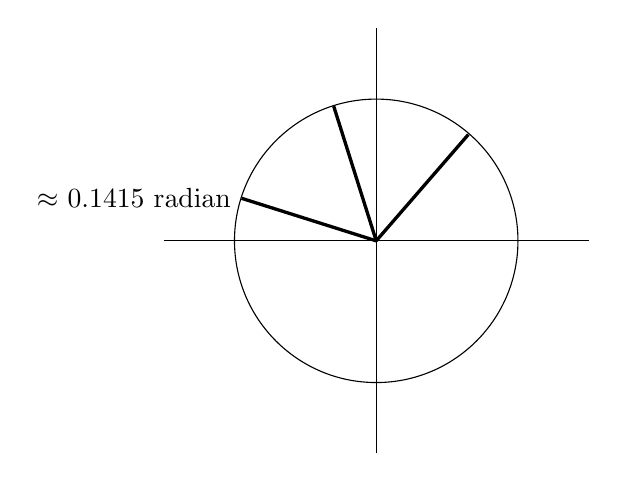
\begin{tikzpicture}[scale=0.9]
		\draw[-] (-3,0) -- (3,0);
		\draw[-] (0,-3) -- (0,3);
		\draw (2,0) arc (0:360:2);
		\draw[-,very thick] (0, 0) -- (1.3, 1.5);
		\draw[-,very thick] (0, 0) -- (-0.6, 1.9);
		\draw[-,very thick] (0, 0) -- (-1.9, 0.6) node[left] {$ \approx $ 0.1415 radian};
	\end{tikzpicture}
	\caption{radian}
\end{figure}

\begin{theorem}[Degrees and radians]
	\begin{align}
		 & 180^\circ = \pi \ radians           \\
		 & 1^\circ = {\pi \over 180} \ radians \\
		 & 1 \ radian = {180 \over \pi}^\circ
	\end{align}
\end{theorem}

This relationship provides us with a way to easily convert between the two measures. \\

\begin{exercise}
	Convert from degrees to radians. \\

	(a) $ 30^\circ = $ \\

	(b) $ 220^\circ = $ 
\end{exercise}

\begin{exercise}
	Convert from radians to degrees. \\

	(a) $ {\pi \over 4} = $ \\

	(b) $ {5\pi \over 6} = $
\end{exercise}

Given any angle $ \theta $, what are these equivalent angles? \\

\begin{theorem}[Equivalent angles]
	\begin{align}
		 & \theta + 2k\pi \ (k \in \mathbb Z)
	\end{align}
\end{theorem}

\chapter{Trigonometric Functions}

\section{Trigonometric Functions}

Let $ O $ be the origin and $ P(x, y) $ be a point on the unit circle so that the radius $ OP $ forms an angle of $ \theta $ radians with respect to the positive x-axis. \\

\begin{figure}[H]
	\centering
	\begin{tikzpicture}[scale=0.9]
		\draw[-] (-3,0) -- (3,0);
		\draw[-] (0,-3) -- (0,3);
		\draw (2,0) arc (0:360:2);
		\draw[-,very thick] (0, 0) -- (1.4, 1.4);
		\draw[-,very thick] (0, 0) -- (1.4, 0);
		\draw[-,very thick] (1.4, 0) -- (1.4, 1.4);
	\end{tikzpicture}
	\caption{radian}
\end{figure}

\begin{theorem}[sin / cos]\nonumber
	\begin{align}
		 & x = cos(\theta) \\
		 & y = sin(\theta)
	\end{align}
\end{theorem}

Here are the three most common trigonometric functions and their reciprocals. \\

\begin{figure}[H]
	\centering
	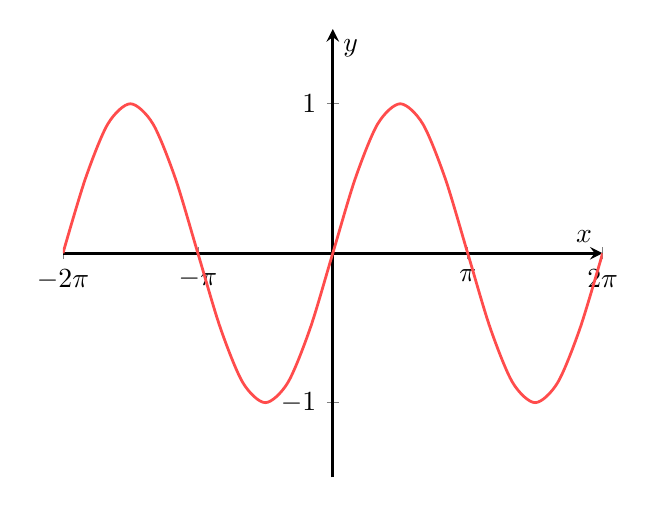
\begin{tikzpicture}
		\begin{axis}[
				xlabel={$ x $}, ylabel={$ y $},
				xmin=-2*pi, xmax=2*pi,
				ymin=-1.5, ymax=1.5,
				xtick={-6.28319, -3.14159, 0, 3.14159, 6.28319},
				xticklabels={$-2\pi$, $-\pi$, $0$, $\pi$, $2\pi$},
				line width=1pt,
				axis lines=center,
			]
			\addplot[smooth,domain=-2*pi:2*pi, red!70]{sin(deg(x))};
		\end{axis}
	\end{tikzpicture}
\end{figure}

\begin{figure}[H]
	\centering
	\begin{tabular}{|c|c|}
		\hline
		range                    & $ -1 \le sin(\theta) \ge 1 $        \\
		\hline
		doamin                   & $ \theta \in \mathbb R $            \\
		\hline
		$ sin(\theta) = 0 $ when & $ \theta = k\pi,\ k \in \mathbb Z $ \\
		\hline
	\end{tabular}
	\caption{$ y = sin(\theta) $}
\end{figure}

\begin{figure}[H]
	\centering
	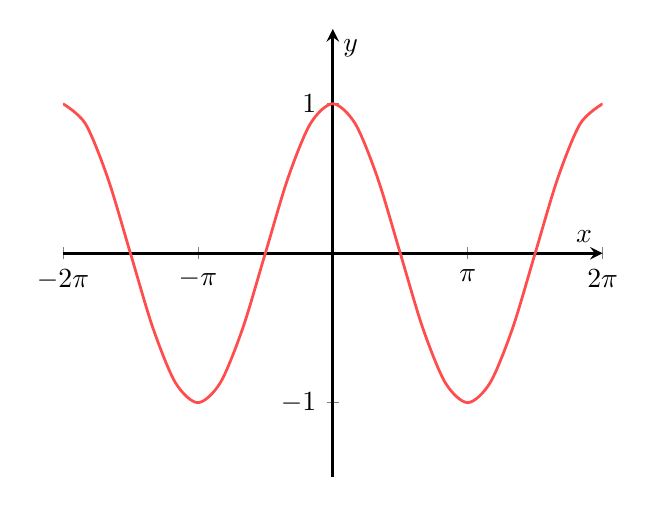
\begin{tikzpicture}
		\begin{axis}[
				xlabel={$ x $}, ylabel={$ y $},
				xmin=-2*pi, xmax=2*pi,
				ymin=-1.5, ymax=1.5,
				xtick={-6.28319, -3.14159, 0, 3.14159, 6.28319},
				xticklabels={$-2\pi$, $-\pi$, $0$, $\pi$, $2\pi$},
				line width=1pt,
				axis lines=center,
			]
			\addplot[smooth,domain=-2*pi:2*pi, red!70]{cos(deg(x))};
		\end{axis}
	\end{tikzpicture}
\end{figure}

\begin{figure}[H]
	\centering
	\begin{tabular}{|c|c|}
		\hline
		range                    & $ \theta \in \mathbb R $                           \\
		\hline
		doamin                   & $ -1 \le cos(\theta) \le 1 $                       \\
		\hline
		$ cos(\theta) = 0 $ when & $ \theta = {(2k+1)\pi \over 2},\ k \in \mathbb Z $ \\
		\hline
	\end{tabular}
	\caption{$ y = cos(\theta) $}
\end{figure}

\begin{figure}[H]
	\centering
	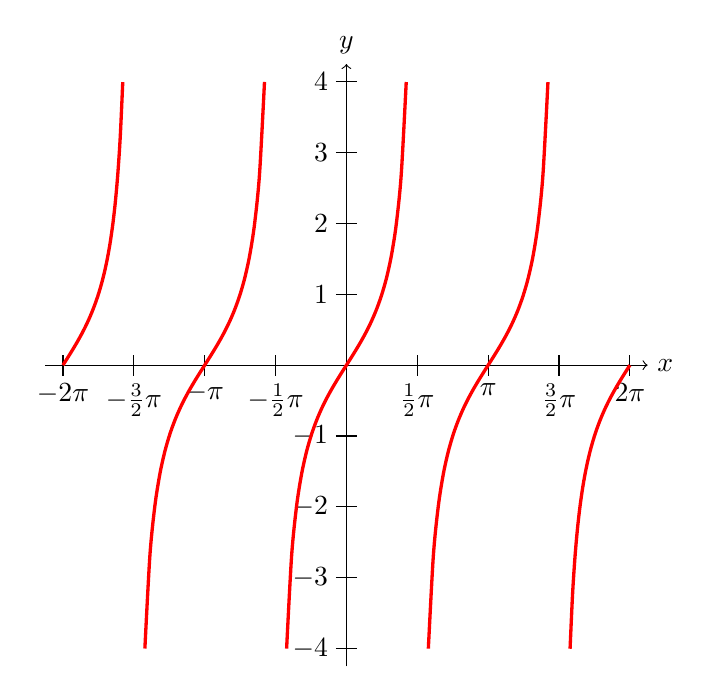
\begin{tikzpicture}[scale=0.9]
		\foreach \x / \r in {-4/-2\pi,-3/-\frac{3}{2}\pi,-2/-\pi,-1/-\frac{1}{2}\pi,1/\frac{1}{2}\pi,2/\pi,3/\frac{3}{2}\pi,4/2\pi} \draw (\x,-0.15) -- (\x,+0.15) node[below=7] {$\r$};
		\foreach \y in {-4,-3,-2,-1,1,2,3,4} \draw (-0.15,\y) -- (+0.15,\y) node[left=7] {$\y$};
		\draw[->] (-4.25,0)--(4.25,0) node[right] {$ x $};
		\draw[->] (0,-4.25)--(0,4.25) node[above] {$ y $};
		\foreach \i in {0,...,4} \draw[very thick,color=red] plot [domain={((\i-2)*pi-rad(atan(4))*ceil(\i/4))*(2/pi)}:{((\i-2)*pi+rad(atan(4))*ceil((4-\i)/4))*(2/pi)},smooth] (\x,{tan(\x*pi/2 r)});
	\end{tikzpicture}
\end{figure}

\begin{figure}[H]
	\centering
	\begin{tabular}{|c|c|}
		\hline
		range                    & $ \theta \in \mathbb R, \theta \ne {(2k+1)\pi \over 2}, k \in \mathbb Z $ \\
		\hline
		doamin                   & $ tan(\theta) \in \mathbb R $                                             \\
		\hline
		$ tan(\theta) = 0 $ when & $ \theta = k\pi,\ k \in \mathbb Z $                                       \\
		\hline
	\end{tabular}
	\caption{$ y = tan(\theta) $}
\end{figure}

\begin{figure}[H]
	\centering
	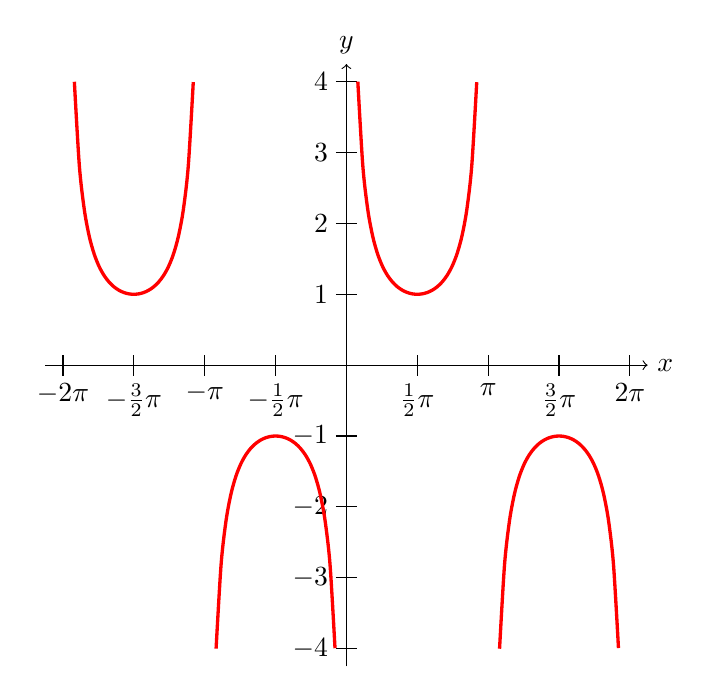
\begin{tikzpicture}[scale=0.9]
		\foreach \x / \r in {-4/-2\pi,-3/-\frac{3}{2}\pi,-2/-\pi,-1/-\frac{1}{2}\pi,1/\frac{1}{2}\pi,2/\pi,3/\frac{3}{2}\pi,4/2\pi} \draw (\x,-0.15) -- (\x,+0.15) node[below=7] {$\r$};
		\foreach \y in {-4,-3,-2,-1,1,2,3,4} \draw (-0.15,\y) -- (+0.15,\y) node[left=7] {$\y$};
		\draw[->] (-4.25,0)--(4.25,0) node[right] {$ x $};
		\draw[->] (0,-4.25)--(0,4.25) node[above] {$ y $};
		\foreach \i in {0,...,3} \draw[very thick,color=red] plot [domain={((\i-2)*pi+rad(asin(1/4)))*(2/pi)}:{((\i-1)*pi-rad(asin(1/4)))*(2/pi)},smooth] (\x,{cosec(\x*pi/2 r)});
	\end{tikzpicture}
\end{figure}

\begin{figure}[H]
	\centering
	\begin{tabular}{|c|c|}
		\hline
		range                    & $ \theta \in \mathbb R,\ \theta \ne k\pi,\ k \in \mathbb Z $ \\
		\hline
		doamin                   & $ csc(\theta) \ge 1 $ or $ csc(\theta) \le -1 $              \\
		\hline
		$ csc(\theta) = 0 $ when & $ never $                                                    \\
		\hline
	\end{tabular}
	\caption{$ y = csc(\theta) $}
\end{figure}

\begin{figure}[H]
	\centering
	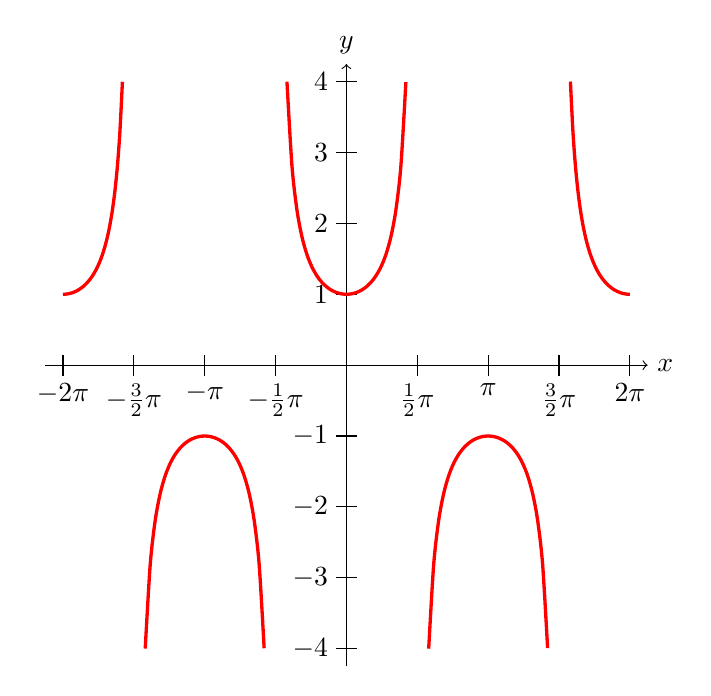
\begin{tikzpicture}[scale=0.9]
		\foreach \x / \r in {-4/-2\pi,-3/-\frac{3}{2}\pi,-2/-\pi,-1/-\frac{1}{2}\pi,1/\frac{1}{2}\pi,2/\pi,3/\frac{3}{2}\pi,4/2\pi} \draw (\x,-0.15) -- (\x,+0.15) node[below=7] {$\r$};
		\foreach \y in {-4,-3,-2,-1,1,2,3,4} \draw (-0.15,\y) -- (+0.15,\y) node[left=7] {$\y$};
		\draw[->] (-4.25,0)--(4.25,0) node[right] {$ x $};
		\draw[->] (0,-4.25)--(0,4.25) node[above] {$ y $};
		\foreach \i in {0,...,4} \draw[very thick,color=red] plot [domain={((\i-2)*pi-rad(acos(1/4))*ceil(\i/4))*(2/pi)}:{((\i-2)*pi+rad(acos(1/4))*ceil((4-\i)/4))*(2/pi)},smooth] (\x,{sec(\x*pi/2 r)});
	\end{tikzpicture}
\end{figure}

\begin{figure}[H]
	\centering
	\begin{tabular}{|c|c|}
		\hline
		range                    & $ \theta \in \mathbb R,\ \theta \ne {(2k+1)\pi \over 2},\ k \in \mathbb Z $ \\
		\hline
		doamin                   & $ sec(\theta) \ge 1 $ or $ sec(\theta) \le -1 $                             \\
		\hline
		$ sec(\theta) = 0 $ when & $ never $                                                                   \\
		\hline
	\end{tabular}
	\caption{$ y = sec(\theta) $}
\end{figure}

\begin{figure}[H]
	\centering
	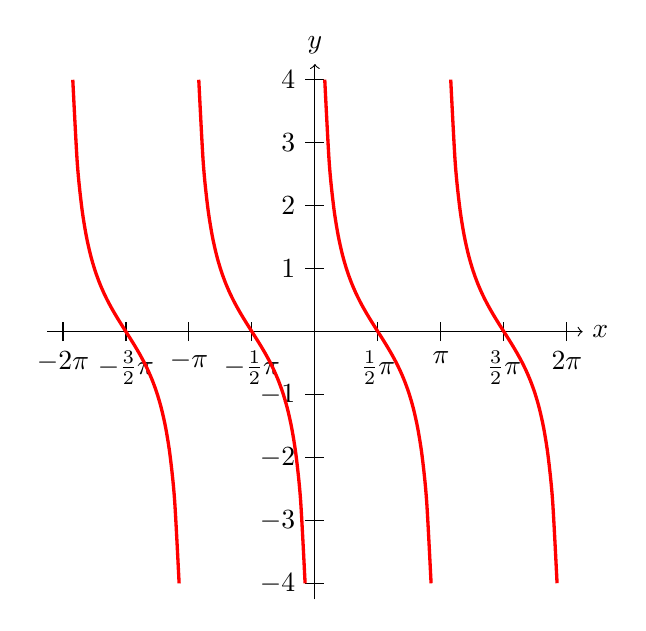
\begin{tikzpicture}[scale=0.8]
		\foreach \x / \r in {-4/-2\pi,-3/-\frac{3}{2}\pi,-2/-\pi,-1/-\frac{1}{2}\pi,1/\frac{1}{2}\pi,2/\pi,3/\frac{3}{2}\pi,4/2\pi} \draw (\x,-0.15) -- (\x,+0.15) node[below=7] {$\r$};
		\foreach \y in {-4,-3,-2,-1,1,2,3,4} \draw (-0.15,\y) -- (+0.15,\y) node[left=7] {$\y$};
		\draw[->] (-4.25,0)--(4.25,0) node[right] {$ x $};
		\draw[->] (0,-4.25)--(0,4.25) node[above] {$ y $};
		\foreach \i in {0,...,3} \draw[very thick,color=red] plot [domain={((\i-2)*pi+rad(atan(1/4)))*(2/pi)}:{((\i-1)*pi-rad(atan(1/4)))*(2/pi)},smooth] (\x,{cot(\x*pi/2 r)});
	\end{tikzpicture}
\end{figure}

\begin{figure}[H]
	\centering
	\begin{tabular}{|c|c|}
		\hline
		range                    & $ \theta \in \mathbb R,\ \theta \ne k\pi, k \in \mathbb Z $ \\
		\hline
		doamin                   & $ cot(\theta) \in \mathbb R $                               \\
		\hline
		$ cot(\theta) = 0 $ when & $ \theta = {(2k+1)\pi \over 2},\ k \in \mathbb Z $          \\
		\hline
	\end{tabular}
	\caption{$ y = cot(\theta) $}
\end{figure}

\section{Special Triangles}

\begin{figure}[H]
	\centering
	\begin{tikzpicture}[scale=0.8]
		\draw (0,0) node[anchor=north]{$ A $}
		-- (4,0) node[anchor=north]{$ C $}
		-- (4,4) node[anchor=south]{$ B $}
		-- cycle;
	\end{tikzpicture}
\end{figure}

\begin{figure}[H]
	\centering
	\begin{tikzpicture}[scale=0.8]
		\draw (0,0) node[anchor=north]{$ A $}
		-- (7,0) node[anchor=north]{$ C $}
		-- (7,3) node[anchor=south]{$ B $}
		-- cycle;
	\end{tikzpicture}
\end{figure}

\begin{exercise}
	Evaluate each of the following. \\

	(a) $ sin({\pi \over 4}) = $ \\

	(b) $ cos({\pi \over 4}) = $ \\

	(c) $ csc({\pi \over 4}) = $
\end{exercise}

\begin{exercise}
	Find all values of $ \theta $ satisfying the following. \\

	(a) $ tan(\theta) = {1 \over \sqrt{3}} $ \\
	\\
	\\

	(b) $ sec(\theta) = \sqrt{2} $ \\
	\\
	\\

	(c) $ cot(\theta) = \sqrt{3} $ \\
	\\
	\\
\end{exercise}

\section{Trigonometric Identities}

\begin{theorem}[Trigonometric Identities]
	\begin{align}
		 & sin^2(\theta) + cos^2(\theta) = 1                    \\
		 & sin(-\theta) = -sin(\theta)                          \\
		 & cos(-\theta) = -cos(\theta)                          \\
		 & tan(\theta) = {sin(\theta) \over cos(\theta)}        \\
		 & cot(\theta) = {cos(\theta) \over sin(\theta)}        \\
		 & tan^2(\theta) + 1 = sec^2(\theta)                    \\
		 & cot^2(\theta) + 1 = csc^2(\theta)                    \\
		 & sin(\theta) = cos\left(\theta - {\pi \over 2}\right) \\
		 & sin(a \pm b) = sin(a)cos(b) \pm cos(a)sin(b)         \\
		 & cos(a \pm b) = cos(a)cos(b) \mp sin(a)sin(b)         \\
		 & sin(2\theta) = 2sin(\theta)cos(\theta)               \\
		 & cos(2\theta) = cos^2(\theta) - sin^2(\theta)         \\
		 & sin^2(\theta) = {1 - cos(2\theta) \over 2}           \\
		 & cos^2(\theta) = {1 + cos(2\theta) \over 2}
	\end{align}
\end{theorem}

Reminder: $ trig^n(x) $ is a notation often used to indicate $ (trig(x))^n $. \\

\chapter{Exponential Functions}

\section{Exponential Functions}

Exponential functions are of the form $ y = a^x $, where $ a $ is a positive number and $ x $ is any real number. You might see these sorts of functions when studying population growth, economic growth, global temperature, monetary value, etc. \\

\begin{figure}[H]
	\centering
	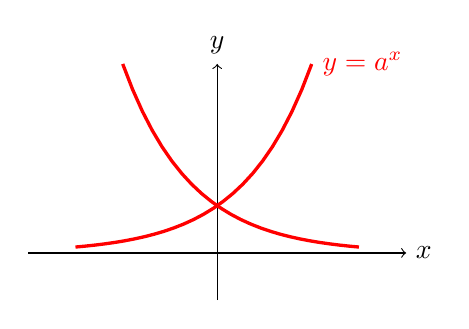
\begin{tikzpicture}[scale=0.6]
		\draw[->] (-4,0) -- (4,0) node[right] {$ x $};
		\draw[->] (0,-1) -- (0,4) node[above] {$ y $};
		\draw[very thick,color=red,domain=-3:2] plot (\x,{2 ^ \x}) node[right] {$ y = {a^x} $};
		\draw[very thick,color=red,domain=-2:3] plot (\x,{0.5 ^ \x});
	\end{tikzpicture}
	\caption{exponential function}
\end{figure}

\begin{itemize}
	\item
	      Domain: $ x \in \mathbb R $ \\

	\item
	      Range: $ y > 0 $ \\

	\item
	      The graph $ y = a^x $ always passes through $ (0, 1) $ and $ (1, a) $. \\

	\item
	      If $ a > 1$ then the graph of $ y = a^x $ is increasing. \\

	\item
	      If $ 0 < a < 1 $ then the graph of  $ y = a^x $ is decreasing. \\

	\item
	      $ y = 0 $ is always a horizontal asymptote of $ y = a^x $. \\
\end{itemize}

\section{Exponent Rules}

\begin{theorem}[Exponent Rules]
	\begin{align}
		 & a^{-x} = {1 \over a^x}                    \\
		 & {1 \over a^{-x}} = a^x                    \\
		 & (ab)^x = a^xb^x                           \\
		 & ({a \over b})^x = {a^x \over b^x}         \\
		 & a^{kx} = (a^k)^x = (a^x)^k                \\
		 & a^ma^n = a^{m+n}                          \\
		 & {a^m \over a^n} = a^{m-n}                 \\
		 & a^{1/n} = \sqrt[n]{a}                     \\
		 & a^{m/n} = \sqrt[n]{a^m} = (\sqrt[n]{a})^m
	\end{align}
\end{theorem}

\section{The Base e}

A very special exponential function is $ y = e^x $, where $ e $ is just a content with a non-terminating decimal like $ \pi $. \\

$$
	e = 2.718281845...
$$

What is so special about an exponential function with base $ e $? \\

At any point on the graph, the height of the exponential function is equal to the slope of the tangent line to the graph at that point. \\

\begin{figure}[H]
	\centering
	\begin{tikzpicture}[scale=0.6]
		\draw[->] (-4,0) -- (4,0) node[right] {$ x $};
		\draw[->] (0,-3) -- (0,4) node[above] {$ y $};
		\draw[very thick,color=red,domain=-3:1] plot (\x,{e ^ \x}) node[left] {$ y = {e^x} $};
		\draw[very thick,color=blue,domain=-2:2] plot (\x,{\x + 1});
	\end{tikzpicture}
	\caption{$ y = e^x $}
\end{figure}

\chapter{Logarithmic Functions}

\section{Logarithmic Functions}

Logarithms are the inverse of exponential functions. Let $ a > 0$, then we define a logarithm (log) as follows: \\

\begin{theorem}[Logarithmic Functions]
	\begin{align}
		y   & = log_a(x) \\
		a^y & = x
	\end{align}
\end{theorem}

If no base $ a $ is shown, a base of 10 is assumed. \\

For example: \\
$$
	log(x) = log_{10}(x)
$$

\begin{exercise}
	Evaluate each of the following. \\

	(a) $ log_{2}8 = $ \\

	(b) $ log(100) = $ \\

	(c) $ log_{5}{1 \over 25} = $ \\

	(d) $ log_{8}1 = $
\end{exercise}

Since any positive number to the power of 0 is equal to 1, we have the property that $ log_a(1) $, no matter what the base $ a $ is. \\

\begin{figure}[H]
	\centering
	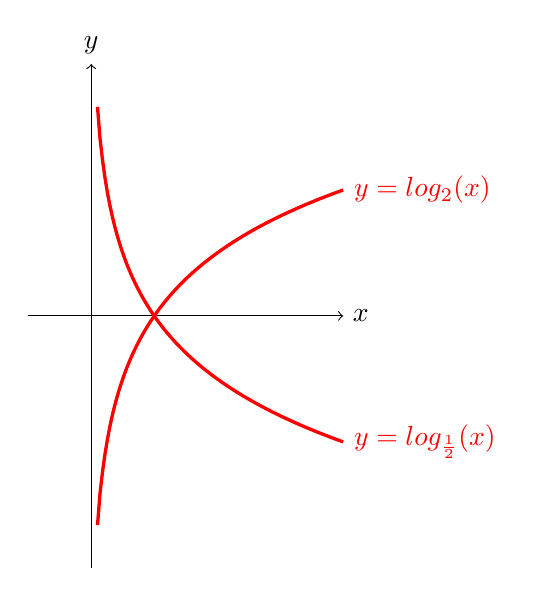
\begin{tikzpicture}[scale=0.8]
		\draw[->] (-1,0) -- (4,0) node[right] {$ x $};
		\draw[->] (0,-4) -- (0,4) node[above] {$ y $};
		\draw [very thick,color=red,domain=0.1:4,samples=100] plot (\x,{log2(\x)}) node[right] {$ y = log_2(x) $};
		\draw [very thick,color=red,domain=0.1:4,samples=100] plot (\x,{log10(\x) / log10(0.5)}) node[right] {$ y = log_{1 \over 2}(x) $};
	\end{tikzpicture}
	\caption{logarithmic function}
\end{figure}

\begin{itemize}
	\item
	      Domain: $ 0 < x < \infty $ \\

	\item
	      Range: $ y \in \mathbb R $ \\

	\item
	      $ y = log_a(x) $ always passes through $ (a, 1) $ and $ (1, 0) $. \\

	\item
	      If $ a > 1 $ then the graph of $ y = log_a(x) $ is increasing. \\

	\item
	      If $ 0 < a < 1 $ then the graph of $ y = log_a(x) $ is decreasing. \\

	\item
	      $ x = 0 $ is always a vertical asymptote of $ y = log_a(x) $. \\
\end{itemize}

\section{Logarithm Rules}

\begin{theorem}[Logarithm Rules]
	\begin{align}
		 & log_a(a^x) = x                                      \\
		 & a^{log_a(x)} = x                                    \\
		 & log_a(xy) = log_a(x) + log_a(y)                     \\
		 & log_a\left({x \over y}\right) = log_a(x) - log_a(y) \\
		 & log_a(x^n) = nlog_a(x)
	\end{align}
\end{theorem}

\section{Change of Base Formula}

We can switch between any two bases easily by using the formula: \\

\begin{theorem}[Change of Base Formula]
	\begin{align}
		log_a(x) = {log_b(x) \over log_b(a)}
	\end{align}
\end{theorem}

\begin{exercise}\nonumber
	Proof
	
	\vspace{5cm}
\end{exercise}

\begin{exercise}\nonumber
	Convert $ log_4(x) $ into a logarithm with each of the following bases. \\

	(a) base 3
	\\
	\\

	(b) base 22
	\\
	\\
\end{exercise}

\section{The Natural Logarithm}

A special logarithm is the natural logarithm, which is the logarithm with a base of $ e $. Rather than write $ log_e(x) $, we typically write $ ln(x) $. \\

The natural logarithm has the exact same properties as any other logarithmic function. \\

\begin{theorem}[Natural Logarithm]
	\begin{align}
		 & ln(e^x) = x   \\
		 & e^{ln(x)} = x
	\end{align}
\end{theorem}

\begin{exercise}\nonumber
	Solve each of the following for $ x $. \\

	(a)
	\begin{align}
		2^x & = 2^{1-x}     \\
		\\
		\\
		\\
	\end{align}
	\\

	(b)
	\begin{align}
		3^{{1 \over 2} + 10} & = 27   \\
		\\
		\\
		\\
		\\
	\end{align}
	\\

	(c)
	\begin{align}
		2^x     & = 10                   \\
		\\
		\\
		\\
		\\
	\end{align}
	\\

	(d)
	\begin{align}
		log(x) - 1   & = log(x - 1)                           \\
		\\
		\\
		\\
		\\
		\\
		\\
		\\
	\end{align}
	\\

	(e)
	\begin{align}
		log_2(x) + log_2(x^2) & = 6 \\
		\\
		\\
		\\
		\\
		\\
	\end{align}
	\\

	(f)
	\begin{align}
		log_2(x^4) + log_2(x^2) & = 6     \\
		\\
		\\
		\\
		\\
		\\
	\end{align}
\end{exercise}